\documentclass[convert={outext=.tex.png}]{standalone}
\usepackage{ulem,tikz,xcolor}
\usetikzlibrary{arrows,arrows.meta,calc,fit,positioning,shapes.geometric}


\begin{document}
%\pagecolor[RGB]{255,255,254}
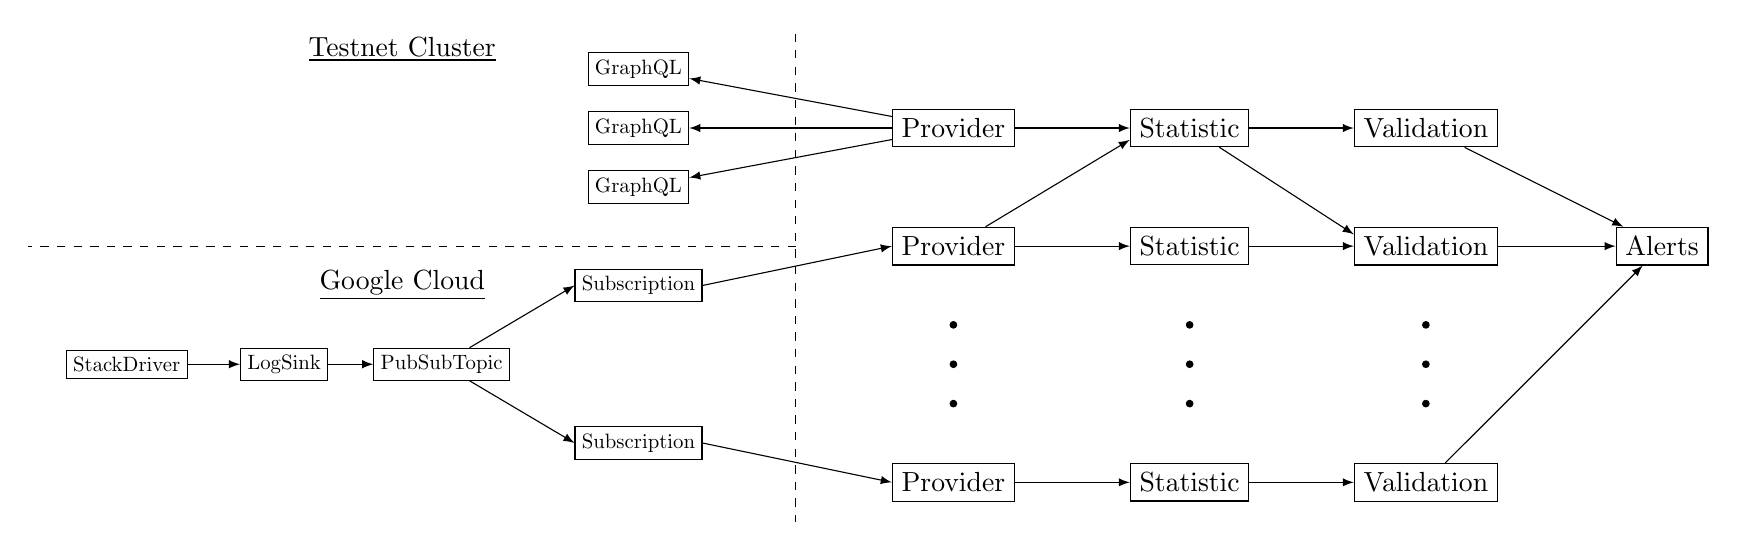
\begin{tikzpicture}
  \foreach \i/\y in {1/-0.75,2/0,3/0.75}
    \node[draw,scale=0.75] (GraphQL-\i) at (-2,\y) {GraphQL};

  \node[draw,scale=0.75] (StackDriver) at (-8.5,-3) {StackDriver};
  \node[draw,scale=0.75] (LogSink) at (-6.5,-3) {LogSink};
  \node[draw,scale=0.75] (PubSubTopic) at (-4.5,-3) {PubSubTopic};
  \node[draw,scale=0.75] (Subscription-1) at (-2,-2) {Subscription};
  \node[draw,scale=0.75] (Subscription-2) at (-2,-4) {Subscription};

  \node at (-5,-2) {\underline{Google Cloud}};
  \node at (-5,1) {\underline{Testnet Cluster}};

  \foreach \x/\role in {2/Provider,5/Statistic,8/Validation} {
    \foreach \i/\y in {1/0,2/-1.5,3/-4.5} {
      \node[draw] (\role-\i) at (\x,\y) {\role};
    }
    \foreach \s in {-0.5,0,0.5} {
      \node[draw,fill,circle,scale=0.25] at (\x,-3-\s) {};
    }
  }

  \node[draw] (Alerts) at (11,-1.5) {Alerts};

  \draw[dashed] (0,1.2) -- (0,-5);
  \draw[dashed] (0,-1.5) -- (-9.75,-1.5);

  \draw[-latex] (StackDriver) -- (LogSink);
  \draw[-latex] (LogSink) -- (PubSubTopic);
  \draw[-latex] (PubSubTopic) -- (Subscription-1.west);
  \draw[-latex] (PubSubTopic) -- (Subscription-2.west);
  \draw[-latex] (Subscription-1.east) -- (Provider-2.west);
  \draw[-latex] (Subscription-2.east) -- (Provider-3.west);
  \foreach \i in {1,2,3} \draw[-latex] (Provider-1) -- (GraphQL-\i);
  \draw[-latex] (Provider-1) -- (Statistic-1);
  \draw[-latex] (Provider-2) -- ($(Statistic-1.west) - (0,0.15)$);
  \draw[-latex] (Provider-2) -- (Statistic-2);
  \draw[-latex] (Provider-3) -- (Statistic-3);
  \draw[-latex] (Statistic-1) -- (Validation-1);
  \draw[-latex] (Statistic-1) -- ($(Validation-2.west) + (0,0.15)$);
  \draw[-latex] (Statistic-2) -- (Validation-2);
  \draw[-latex] (Statistic-3) -- (Validation-3);
  \foreach \i in {1,2,3} \draw[-latex] (Validation-\i) -- (Alerts);
\end{tikzpicture}
\end{document}
